\section{Results and comparison}
%
% REMARK. testcases are run for about 900 seconds. iter/sec was taken from the last entry
%         started with ./nltool -i ../hash/sha2/chars/sha256/startchars/27-t10.xml
%         SAT_EXPLICIT_SOLUTION must be disabled in every branch.
%
%\begin{table}[t]
\begin{sidewaystable}
 \begin{center}
  \begin{tabular}{lccccc}
                               & \multicolumn{3}{c}{1 additional bit condition requires in average} & \\
   Approach                    & boolean vars & clauses & assumptions   & performance \\
  \hline
   % lp/sat-se: Info: seed: 2578791537 time: 886 iterations/sec: 0 iterations: 568 stack_size: 4 contr: 38 restarts: 1 minfree: 105 absminfree: 105 credits: 9962 phase: 0 found: 0 smax: 9 complete: 0/0 
   % lp/sat-se: Info: seed: 2578791537 time: 888 iterations/sec: 0 iterations: 569 stack_size: 4 contr: 38 restarts: 1 minfree: 105 absminfree: 105 credits: 9962 phase: 0 found: 0 smax: 9 complete: 0/0 
   Simple evaluation           & $2.0$        & $1.375$ & $0$           & $0$ iter/sec \\
   % lp/sat-al: Info: seed: 1124351917 time: 887 iterations/sec: 23 iterations: 130 stack_size: 0 contr: 3 restarts: 63 minfree: 160 absminfree: 44 credits: 9997 phase: 0 found: 0 smax: 3 complete: 0/0 
   % lp/sat-al: Info: seed: 1124351917 time: 889 iterations/sec: 23 iterations: 38 stack_size: 1 contr: 0 restarts: 64 minfree: 315 absminfree: 44 credits: 10000 phase: 0 found: 0 smax: 1 complete: 0/0 
   %
   % lp/sat-al: Info: seed: 1124351917 time: 895 iterations/sec: 23 iterations: 113 stack_size: 4 contr: 0 restarts: 65 minfree: 197 absminfree: 44 credits: 10000 phase: 0 found: 0 smax: 4 complete: 0/0 
   % lp/sat-al: Info: seed: 1124351917 time: 897 iterations/sec: 23 iterations: 61 stack_size: 1 contr: 0 restarts: 66 minfree: 276 absminfree: 44 credits: 10000 phase: 0 found: 0 smax: 1 complete: 0/0
   Activation literals         & $7.0$        & $6$     & $5.6875$      & $\approx23$ iter/sec \\
   Exhaustive encoding         & $17$         & $46$    & $1$           & N/A \\
   % lp/sat-re: Info: seed: 843358102 time: 886 iterations/sec: 11 iterations: 146 stack_size: 3 contr: 5 restarts: 33 minfree: 159 absminfree: 51 credits: 9995 phase: 0 found: 0 smax: 4 complete: 0/0 
   % lp/sat-re: Info: seed: 843358102 time: 888 iterations/sec: 11 iterations: 171 stack_size: 1 contr: 10 restarts: 33 minfree: 151 absminfree: 51 credits: 9990 phase: 0 found: 0 smax: 4 complete: 0/0 
   % lp/sat-re: Info: seed: 843358102 time: 890 iterations/sec: 11 iterations: 193 stack_size: 4 contr: 10 restarts: 33 minfree: 151 absminfree: 51 credits: 9990 phase: 0 found: 0 smax: 4 complete: 0/0 
   %
   % lp/sat-re: Info: seed: 843358102 time: 899 iterations/sec: 11 iterations: 315 stack_size: 0 contr: 24 restarts: 33 minfree: 118 absminfree: 51 credits: 9976 phase: 0 found: 0 smax: 5 complete: 0/0 
   % lp/sat-re: Info: seed: 843358102 time: 901 iterations/sec: 11 iterations: 25 stack_size: 1 contr: 0 restarts: 34 minfree: 320 absminfree: 51 credits: 10000 phase: 0 found: 0 smax: 1 complete: 0/0 
   % lp/sat-re: Info: seed: 843358102 time: 903 iterations/sec: 11 iterations: 59 stack_size: 1 contr: 0 restarts: 34 minfree: 286 absminfree: 51 credits: 10000 phase: 0 found: 0 smax: 1 complete: 0/0 
   Reduced encoding            & $9$          & $20$    & $1.25$        & $\approx11$ iter/sec \\
   % lp/sat-dse: Info: seed: 1503521737 time: 894 iterations/sec: 7 iterations: 217 stack_size: 8 contr: 2 restarts: 12 minfree: 162 absminfree: 18 credits: 9998 phase: 0 found: 0 smax: 8 complete: 0/0
   % lp/sat-dse: Info: seed: 1503521737 time: 896 iterations/sec: 7 iterations: 237 stack_size: 4 contr: 10 restarts: 12 minfree: 159 absminfree: 18 credits: 9990 phase: 0 found: 0 smax: 8 complete: 0/0
   % lp/sat-dse: Info: seed: 1503521737 time: 898 iterations/sec: 7 iterations: 262 stack_size: 2 contr: 13 restarts: 12 minfree: 159 absminfree: 18 credits: 9987 phase: 0 found: 0 smax: 8 complete: 0/0
   % lp/sat-dse: Info: seed: 1503521737 time: 900 iterations/sec: 7 iterations: 283 stack_size: 3 contr: 13 restarts: 12 minfree: 159 absminfree: 18 credits: 9987 phase: 0 found: 0 smax: 8 complete: 0/0
   % lp/sat-dse: Info: seed: 1503521737 time: 902 iterations/sec: 7 iterations: 302 stack_size: 1 contr: 16 restarts: 12 minfree: 159 absminfree: 18 credits: 9984 phase: 0 found: 0 smax: 8 complete: 0/0
   Differential state encoding & $4$          & $7$     & $1.5$         & $\approx7$ iter/sec \\
  \end{tabular}
  \caption[All encodings in comparison]{
    All encodings in comparison.
    The number of variables and clauses is not important in the first place, but will influence the SAT solvers performance.
    A small number of assumptions is desirable in any case.
  }
  \label{tab:encoding-cmp}
 \end{center}
%\end{table}
\end{sidewaystable}

Simple evaluation obviously has the worst performance. Destroying and building the SAT solver takes a lot of time and slows down the automated search. The advantage of this approach comes into play, when the evaluated differential characteristic is very large. However this size is not within the scope for SAT-based attacks of hash algorithms.

The approaches for Activation literals, Reduced encoding and Differential state encoding all seem interesting and perform very good. Further study is advised to improve the speed by studying the recurring structures due to assigned bit conditions.

\section{Propagation}
%
The propagation in the automated search improved previous implementation, because overlapping bits are detected and considered. Therefore the implementation scales better for larger sizes, because invalid paths are eliminated faster. Figure~\ref{fig:sat-propagation} can directly be compared to the propagation diagrams given in~\cite{Cry16}.
%
\begin{figure}[t]
 \begin{center}
  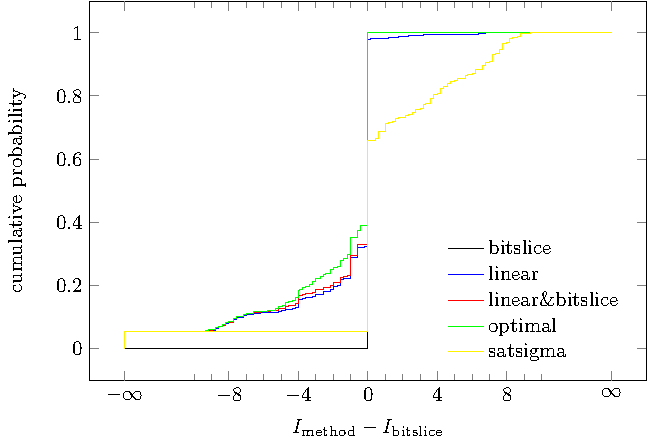
\includegraphics{img/propagation.pdf}
  \caption[Comparison of propagation methods.]{Comparison of propagation methods. Higher values mean better propagation.}
  \label{fig:sat-propagation}
 \end{center}
\end{figure}

\section{Implementation-dependent improvements}
%
\begin{itemize}
  \item Tests shall be made also with different state-of-the-art SAT solvers from different families of the DPLL algorithm such that comparison is possible.
  \item An implementation of the activation literal approach is desirable.
  \item The truth table is a bottleneck of the Initialization step. Tests are required whether approaches like Tseitin's Definitional Normal Form perform better as discussed in~\cite{Sat03}.
  \item SAT solvers themselves propagate values in their evaluation. The same concept is desirable in \nltool. Strategies to put SAT solver technology directly into the framework shall be discussed.
  \item Any fast simplification algorithms for boolean equations are of interest. In the initialization step all clauses are already known. Performing a simplification algorithm especially to the clauses of the primitive functions might lead to a speedup. Karnaugh maps, the Quine-McCluskey algorithm and the Espresso algorithm shall be considered. Simplification algorithms have been implemented by Akawat Homsirikamol et~al.~\cite{Cry04} with HDL in the Quartus II software.
\end{itemize}

\section{Independent approaches}
%
\begin{itemize}
  \item SMT solvers and STP allow a more powerful encoding of the problem to solve. This deprecates the usage of truth tables and encodings. A comparison is of interest.
\end{itemize}
